\section{Networking}
The following section will examine the different possibilities regarding transmitting player position data to the Unity applications used to play the game.

\subsection{Possible networking solutions}
Unity will be used for the creation of the game aspect of this project as described in \autoref{sec:unity-intro}.
Unity includes a proprietary networking solution known as UNet \cite{unityunet}.
This solution allows developers to use a high-level API, giving access to commands that cover many common requirements for multiplayer games, without worrying about the low-level details.
Since the solution is developed alongside the actual game engine, it has a higher level of integration with the Unity Editor and Engine, which allows for certain components and visual aids to aid the building of the game.
As of the beginning of this project, the UNet solution has been deprecated for a while, and the Unity developers are actively working to create a new system to replace it.
The current UNet iteration is usable but will be removed in the future.
Other third-party solutions for Unity-based games also exist, such as Photon Engine.
Photon provides functionality for the developers to make use of to create multiplayer games in the same way as UNet, exposing higher-level functionality.
Photon supports multiple platforms outside of just Unity, with both Android and iOS support \cite{photonnet}.
\\\\
ZeroMQ is also a possible solution.
ZeroMQ is an asynchronous messaging library.
It can carry messages across various transport formats and is available in many different programming languages \cite{zeromqdoc}.
It aims to be a high-performance library to be used in distributed or concurrent applications that are reliable.
According to the getting started guide provided by ZeroMQ, certain issues tend to arise when developers attempt to create a networking solution using sockets \cite{zeromqguide}.
These are:
\begin{itemize}
    \item How to handle I/O?
    \item How are dynamic components handled? What happens if a component disappears temporarily?
    \item How are messages represented? Different sizes and different content can change representations
    \item How are messages that cannot be delivered immediately handled?
    \item Where should message queues be stored?
    \item How are lost messages handled?
    \item What if the network transport changes, for example, TCP to UDP?
    \item How do messages get routed? Can the same message be sent to multiple peers?
    \item How to write an API for another language?
    \item How to represent data such that it can be read between different architectures? How much of this should be the messaging system's job?
    \item How do network errors get handled?
\end{itemize}
These issues are mostly applicable to general solutions that need to accommodate changing requirements or be reusable.
However, for this project, not all of these issues are relevant.
In terms of problems to overcome, this project should only be concerned with handling dynamic components, handling lost messages, routing messages and handling network errors.
If a player closes the game application it can lead to dynamic component issues.
A message can be lost during the playing of the game. 
Messages should be delivered to all players to ensure that they all have the same information.
Finally, a player might suddenly disconnect from the network. 
\\\\
The alternative to making use of a pre-existing solution is creating a custom solution.
A custom solution entails a need to establish a familiarity with the required knowledge to construct such a solution.
A custom solution would involve sockets, which are a network API  that allows programs to communicate with each other \cite{socketnetworking}.

\subsection{Choosing a solution}
There are certain pros and cons associated with both approaches of using either a pre-existing solution or a custom solution.
\autoref{tab:networkprosandcons} shows some of the considerations made when deciding an approach for this project.
\begin{table}[tbp]
    \begin{tabularx}{\textwidth}{|X|X|X|X|}
    \hline
                    & Pre-existing                                                & Custom                                                                            & ZeroMQ                                                                                  \\ \hline
    Customizability & Consists of a set of pre-defined functionalities            & Can have any functionality implemented                                            & Has pre-defined functionalities, but these are lower level than a pre-existing solution \\ \hline
    Requirements    & Familiarity with the solution                               & Familiarity with the knowledge required to implement a usable solution            & Needs familiarity with a mix of pre-existing and custom solutions                     \\ \hline
    Optimization    & Lower-level details are obscured, optimized for general use & Lower-level details are freely available, can be optimized for a specific purpose & Focuses on performance, but the solution is general                                     \\ \hline
    \end{tabularx}
    \caption{A comparison of the pros and cons of the possible solutions}
    \label{tab:networkprosandcons}
\end{table}
Based on these considerations, it was decided that a custom solution should be created to handle networking in this project.
This choice was based on the lack of transparency in a pre-existing solution as well as the need for fast communication.
For the game to be playable and enjoyable, the location data collected by the Pozyx system needs to be transmitted to all the clients as quickly as possible such that they always have an up to date view of the positions of the players.
To achieve this, it would be preferable to build a solution capable of performing the minimum amount of work as quickly as possible.
Pre-existing solutions cannot be guaranteed to do the minimum amount of work as lower-level details are obscured from the developers.
With a custom solution, the data sent across the network can be guaranteed to be exactly what is needed.
ZeroMQ was also a possible choice based on the performance needs, but its generalized approach concerning itself with reusability and issues unlikely to be a big factor in this project meant it was dismissed, in favor of a custom solution in which the problems defined in the previous section are handled.

\subsection{Introduction to sockets}
LAV OG INDSÆT BILLEDE AF OSI LAYER OG HVOR SOCKETS ER :D
Programs that communicate across a computer network need an agreement on how those programs will communicate.
This is known as a protocol.
Generally, before defining the design details of the protocol, a decision should be made as to which program is expected to initiate communication.
One way of defining this is through the client server architecture illustrated in \autoref{fig:client-server}.
This split is used by most network-aware application\cite{socketnetworking}.
The most common method of initiating communication when using the client-server architecture is to have the client initiate requests.
This tends to simplify the protocol and the programs themselves\cite{socketnetworking}.

\begin{figure}[H]
    \centering
    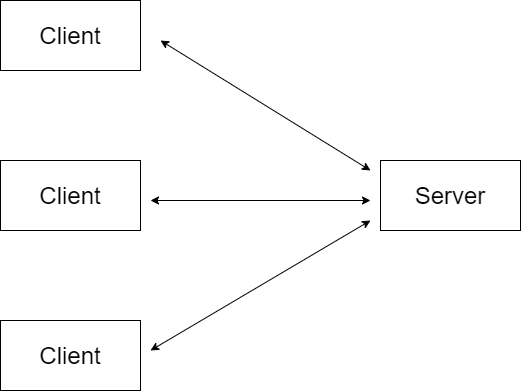
\includegraphics[width=0.6\linewidth]{networking/client_server.png}
    \caption{An illustration of the client-server architecture with multiple clients}
    \label{fig:client-server}
\end{figure}


\subsection{TCP and UDP}
The following section introduces two different protocols for communication - Transmission Control Protocol(TCP) and User Datagram Protocol(UDP).
Both of these protocols use a network-layer protocol known as IP, which can be either the protocol IPv4 or IPv6.

\subsubsection{TCP}
TCP provides connections between clients and servers.
A TCP client establishes a connection with a given server, then it receives or sends data to that server across the network and closes the connection.
TCP provides reliability.
When TCP sends data, it requires an acknowledgement from the receiver that the data has been received.
If it does not receive such an acknowledgement, TCP automatically retransmits the data and then waits for an acknowledgement for the retransmission.
After a certain number of retransmissions TCP gives up.
Based on implementation TCP will typically attempt to send data for 4-10 minutes.
This does not guarantee that the the receiver will receive the data, but the guarantee is that it will deliver the data if possible, or notify the user that the connection has been broken without an acknowledgement from the receiver.
In order to know how long to wait for acknowledgements, TCP contains algorithms to estimate the \textit{round-trip time} between the client and server dynamically.
It also performs these estimations continuously, as the result can be affected by variations in the network traffic.
TCP sequences data by associating bytes and sequence numbers.
For example, if an application writes 2048 bytes to a TCP socket, it would be sent in two segments, with the first containing data with the sequence number 1-1024, and the second containing daa with the sequence number 1025-2048.
If they arrive in the wrong order, the receiving TCP reorders the segments based on the sequence numbers before passing the data to the receiving application.
If the receiver receives duplicate data this can also be detected through the sequence numbers, and the duplicate data can be deleted.
TCP provides flow control by telling clients how many bytes of data can be accepted at any time, known as the window.
The size of the window decreases as data is received, and decreases as the receiver reads data from its buffer.

\subsubsection{UDP}
UDP is a simple transport-layer protocol\cite{socketnetworking}.
An application writes a message to a UDP socket, which gets encapsulated in a UDP datagram, which further gets encapsulated in an IP datagram and then sent to the destination.
A UDP datagram is not guaranteed to reach its final destination, nor is it guaranteed that order will be preserved across the network, or that datagrams arrive only once.
This means that the UDP protocol is unreliable.
If a datagram is lost on the network and not delivered to the UDP socket, it will not be automatically retransmitted.
UDP also does not provide acknowledgement that datagrams were received, sequence numbers to ensure data can be ordered, \textit{round-trip time} estimation or timeouts.
UDP has no notion of flow control, meaning it is possible for a fast UDP sender to transmit data at a rate the receiver is unable to keep up with.
As such, it does not provide the same reliability as TCP.
If reliability is a requirement, it has to be built through features such as timeouts, retransmissions and adding acknowledgements from the receiving end.
A UDP datagram has a length, which is passed to the receiving application along with the data.
UDP is considered connectionless, as there does not need to be a long-term relationship between a UDP client and the server.
A UDP client can create a socket and send a datagram to a server, and then immediately send another datagram on the same socket to a different server.
A UDP server can receive several datagrams on a single UDP socket, each from different clients.


\subsubsection{Choosing between UDP or TCP}
Windowed flow control might not be necessary for transactions where both ends agree on the maximum size of a request or a reply.
For this project only one type of message will be sent - the player location data.
This message will always be formatted in the same way, and as such, a maximum size can be agreed meaning the flow control aspecot of TCP is not needed.

section 22.4
section 21
